\documentclass[utf8,usehyperref,12pt]{G7-32}
\usepackage[T2A]{fontenc}
\usepackage[utf8]{inputenc} %% ваша любимая кодировка здесь
\usepackage[russian]{babel} %% это необходимо для включения переносов
\usepackage{float}
\usepackage{textcase} 
\usepackage{lastpage}
\usepackage[dvips]{graphicx}
\graphicspath{{pictures/}}
\DeclareGraphicsRule{*}{eps}{*}{}
\TableInChaper % таблицы будут нумероваться в пределах раздела
\PicInChaper   % рисунки будут нумероваться в пределах раздела
\setlength\GostItemGap{2mm}% для красоты можно менять от~0мм

% Определяем заголовки для титульной страницы
\NirOrgLongName{
Министерство общего и профессионального образования РФ

\MakeUppercase{Санкт-петербургский государственный университет информационных технологий, механики и оптики}
}
%\NirBoss{Научный руководитель}{И.И.Упырёв} %% Заказчик, утверждающийНИР
\NirManager{Научный руководитель}{Р.~В.~Иванов} 

\NirYear{2010}%% если нужно поменять год отчёта; если закомментировано, ставитсятекущий год
\NirTown{г. Санкт-Петербург,} %% город, в котором написан отчёт
% по проекту \No8550: 

% \NirIsAnnotacion{АННОТАЦИОННЫЙ } %% Раскомментируйте, если это аннотационный
%отчёт

\NirUdk{УДК \No 2123132123}
\NirGosNo{Регистрационный \No 123123}

%\NirStage{Этап \No 1.1}{промежуточный}{<<Обзор современного состояния торсионных
%наногенераторов>>} %%% Этап НИР: {номер этапа}{вид отчёта - промежуточный или
%заключительный}{название этапа}

\bibliographystyle{unsrt} %Стиль библиографических ссылок БибТеХа

%%%%%%%<------------- НАЧАЛО ДОКУМЕНТА
\begin{document}
\usefont{T2A}{ftm}{m}{} %%% Использование шрифтов Т2 для возможности скопировать
%текст из PDF-файлов.

\frontmatter %%% <-- это выключает нумерацию ВСЕГО; здесь начинаются
%ненумерованные главы типа Исполнители, Обозначения и~прочее

\NirTitle{\textbf{<<Выпускная квалификационная работа>>}}
%%% Название НИР и~генерация титульного листа


\Executors %% Список исполнителей здесь
%% это рисует линию размера 3мм и~толщиной 0.1 пункт
\begin{longtable}{p{0.35\linewidth}p{0.2\linewidth}p{0.35\linewidth}}
Научный руководитель, 	&		&	\\
Р.В.~Иванов	&\rule{1\linewidth}{0.1pt}	&  \\ \vspace{1cm}

Выполнил  &		&	\\
Н.В.~Назаренко, & \rule{1\linewidth}{0.1pt}& \\
\end{longtable}

\Referat %% Реферат отчёта, не~более 1 страницы
Отчёт \pageref{LastPage}~c. 4~рис., 3~табл.

\MakeUppercase{Linux, хранилилище, webdav}



\tableofcontents

%\NormRefs % Нормативные ссылки 
%\Defines % Необходимые определения 



\Introduction

placeholder

\mainmatter %% это включает нумерацию глав и~секций в документе ниже

\chapter{Глава 1. Обзор и техническое задание}

\section{Обзор особенностей заказчика}
\subsection{Организационная структура}
Санкт-петербургский городской дворец творчества юных обладает большой и сложной организационной структурой, для каждого 
элемента которого, характерен свой вид деятельности. Рассмотрим организацию с точки зрения двух аспектов: территориального
и структурного.

Территориальная распределенность обусловленна тем, что Дворц творчества юных расположен в центре города, на его территории находиться множество отдельных корпусов, а также ему принадлежит довольно большой участок земли на Крестовском острове и ЗЦДЮТ «Зеркальный». Доступ пользователей к глобальным и локальным информационным ресурсам обеспечивается подключениями по выделенной линии
(2 мб/с), по оптоволокну (1000 мб/с) и прямыми подключениями к узлу (100 мб/с). Сеть рассчитана на большое количество пользователей ИТ-инфраструктурой (более
15 000 компьютеров). Среди них: работники дворца; педагоги; управляющий персонал;  персонал, отвечающий за сервисную деятельность; учащиеся. Сложность управленческой структуры организации определяется большим штатом сотрудников и широким спектром исполняемых функций. Главным руководителем является генеральный директор, которому подчиняются различные подразделения такие как: финансовый, хозяйственный, учебно-воспитательный и другие сектора.

\begin{figure}[ht]
   \centering%центрируем картинку
   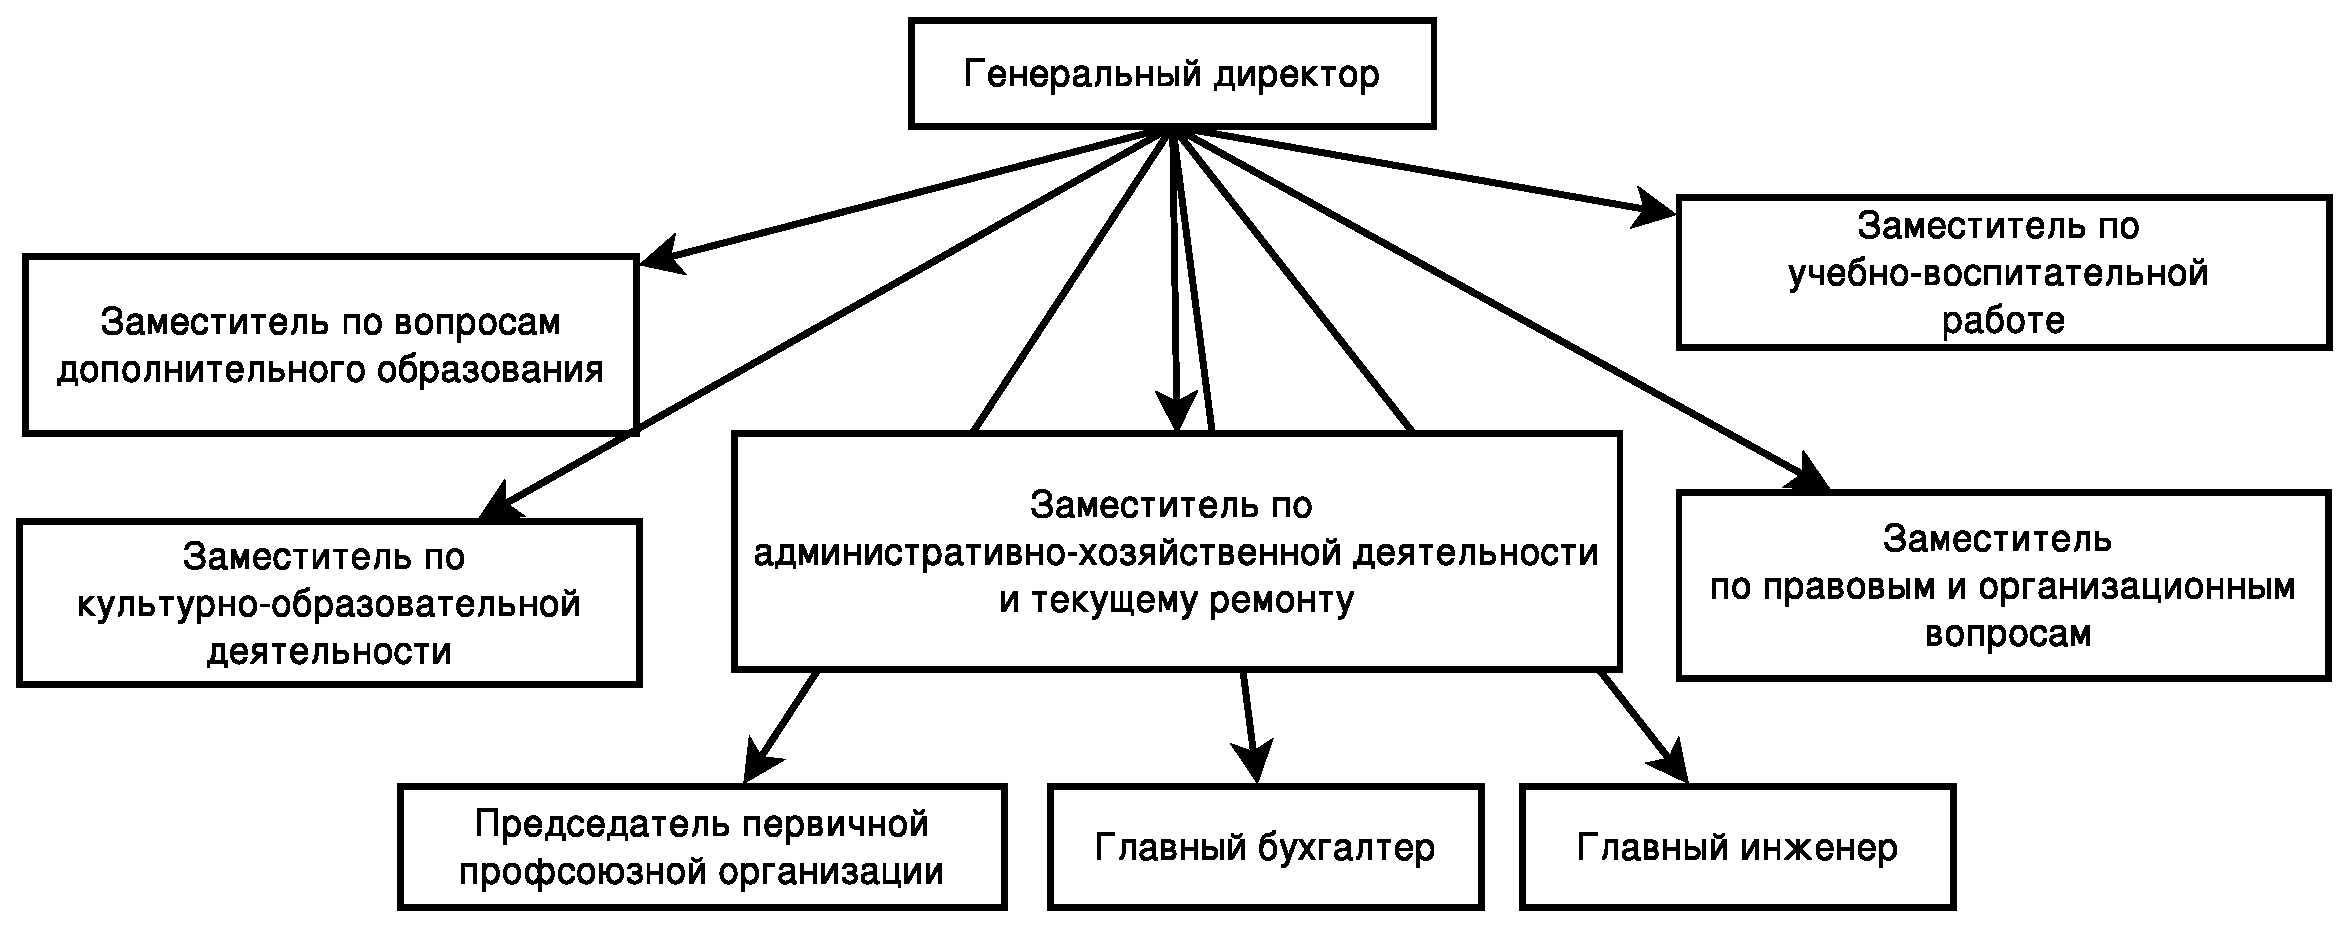
\includegraphics[height=160mm, width=0.8\textwidth, clip, keepaspectratio]{pictures/management_structure.eps}
   \caption{Структура управления организацией}\label{fig:fig_management_struct}
 \end{figure}

\begin{figure}[ht]
   \centering%центрируем картинку
   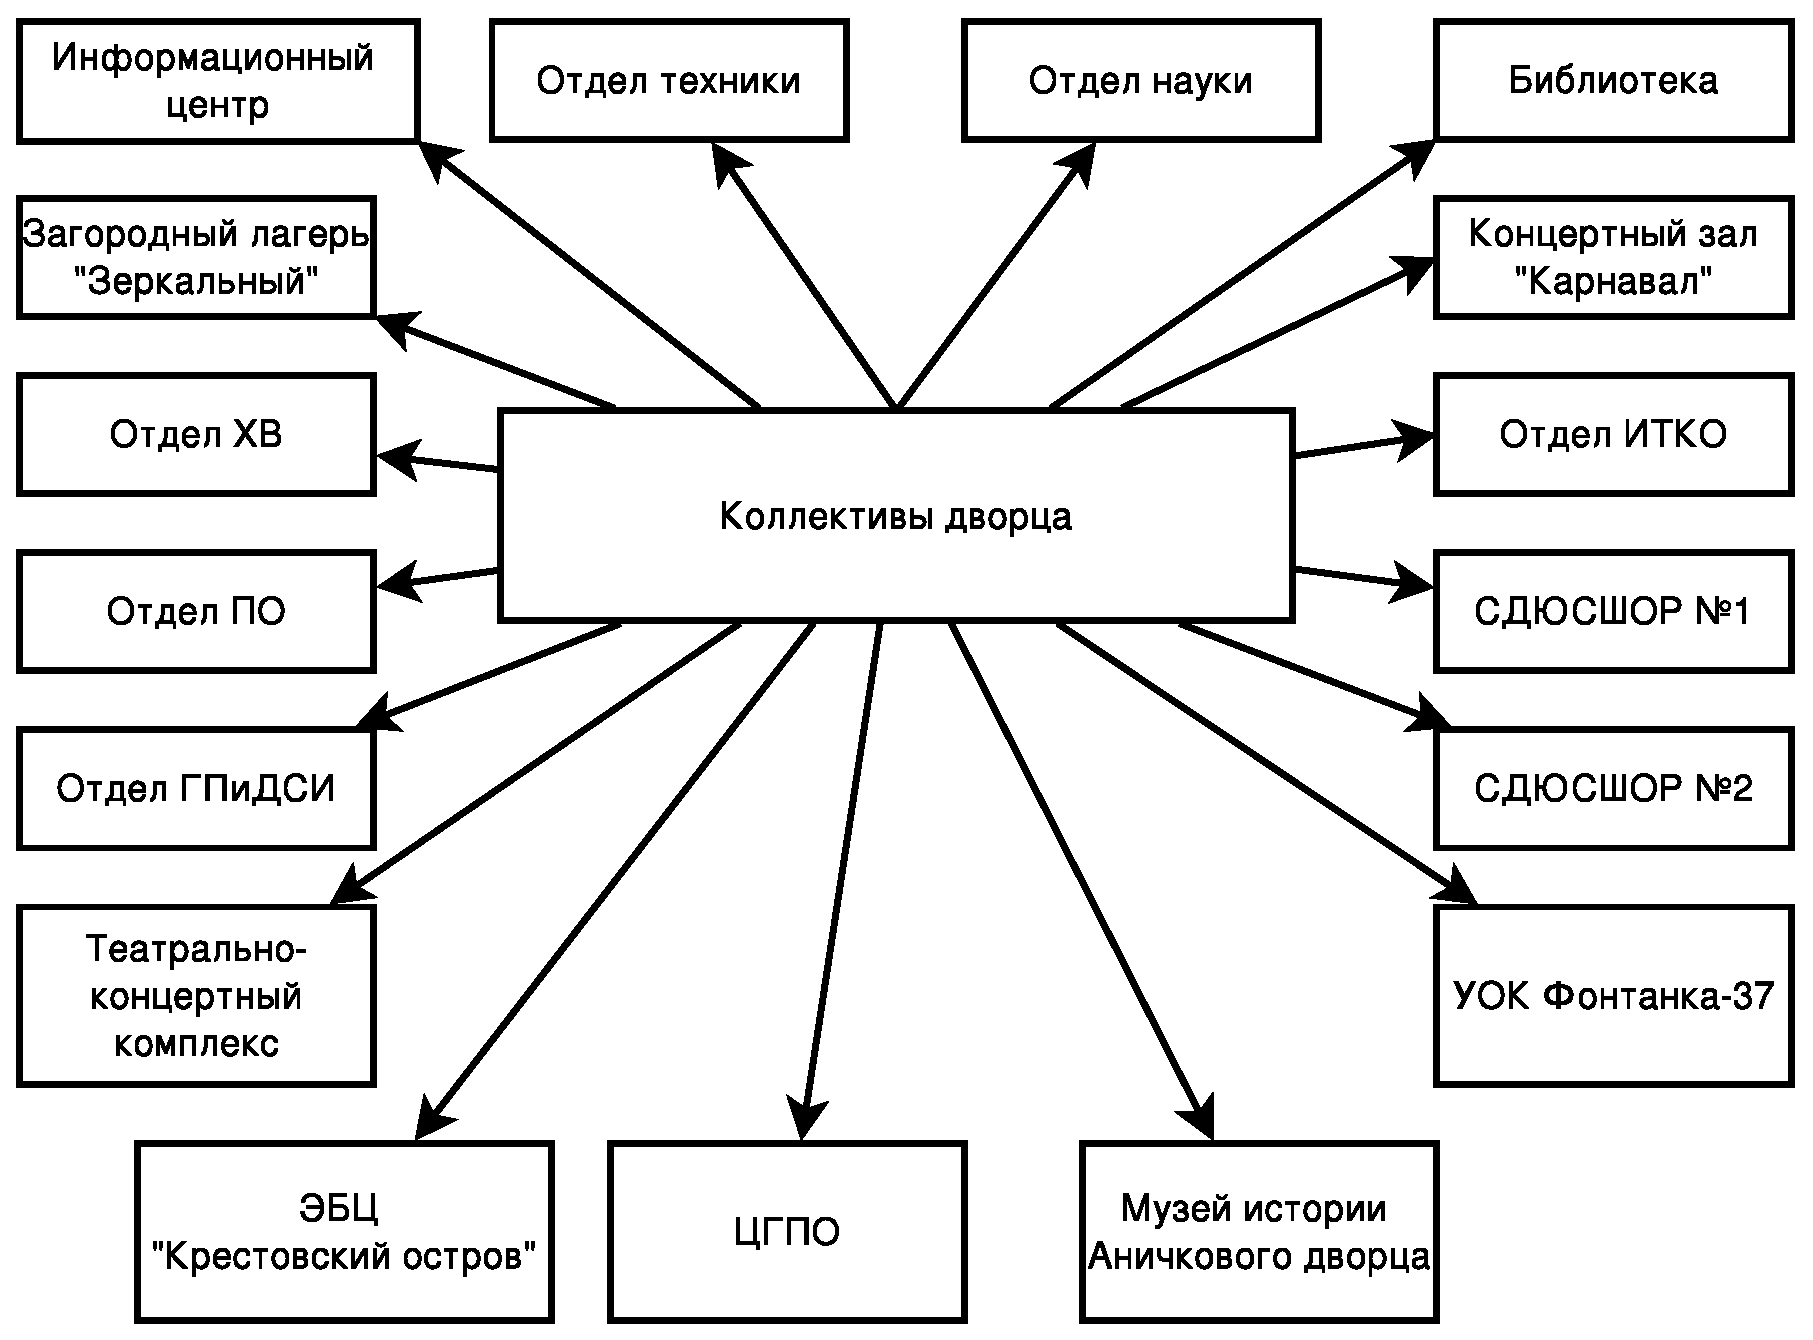
\includegraphics[height=160mm, width=0.8\textwidth, clip, keepaspectratio]{pictures/org_struct.eps}
   \caption{Структура подразделений}\label{fig:org_structure}
 \end{figure}


Сотрудники дворца разделены на коллективы или отделы, отвечающие за определенный вид деятельности(рисунок \ref{fig:org_structure}) 
Каждый отдел в свою очередь имеет большое количество своих подразделений. У каждого коллектива или отдела есть свой директор, один или несколько заместителей и большое количество сотрудников.


\begin{itemize}
\item Отдел ХВ – отдел художественного воспитания
\item Отдел ПО – отдел предшкольного  образования
\item Отдел ГПиДСИ – отдел гуманитарных программ и детских социальных инициатив
\item Отдел ИТКО – отдел информационных технологий и компьютерного обеспечения
\item СДЮС школа №1 – специализированная детско-юношеская спортивная школа №1
\item СДЮС школа № – специализированная детско-юношеская спортивная школа №2
\item УОК <<фонтанка-37>> – учебно-оздоровительный комплекс <<фонтанка-37>>
\item ЭБЦ <<крестовский остров>> – эколого-биологический центр <<крестовский остров>>
\item ЦГПО – центр городских предметных олимпиад.
\end{itemize}

Основной функцией дворца является оказание образовательных и воспитательных услуг, предоставление которых оказывают учебные коллективы, осуществляющие свою деятельность под управлением методических подразделений самого Дворца
и управляющих организаций МОиН города. Кроме непосредственно обучения сотрудники  составляют различные учебные программы, рабочие планы, отчеты, разрабатывают учебно-методические пособия.
Обеспечением текущей деятельности дворца, в аспекте поддержания в надлежащем состоянии оборудования, коммуникаций занимаются сервисные подразделения Дворца. Схема должностей СПБГТЮ представлена на рисунке \ref{fig:fig_management_struct}.

\subsection{Задачи требующие инфраструктурного сопровождения}

хранения результатов работы в понятном как для ИС так и для пользователя виде что решается посредством записи данных в структуру имеющую название файл. 

\subsection{Ограничения накладываемые на информационное сопровождение}
Поскольку организация осуществляет переход на свободное программное обеспечение, то требуется использование исключительно свободных программных продуктов для 
В проекте используются только компоненты распространяющиеся под свободными лицензиями, одобренными OSI(Open Software Initiative). Решение должно функционировать в операционной системе GNU/Linux и быть независимым от ОС установленной на рабочем месте пользователя.

\begin{figure}[ht]
   \centering%центрируем картинку
   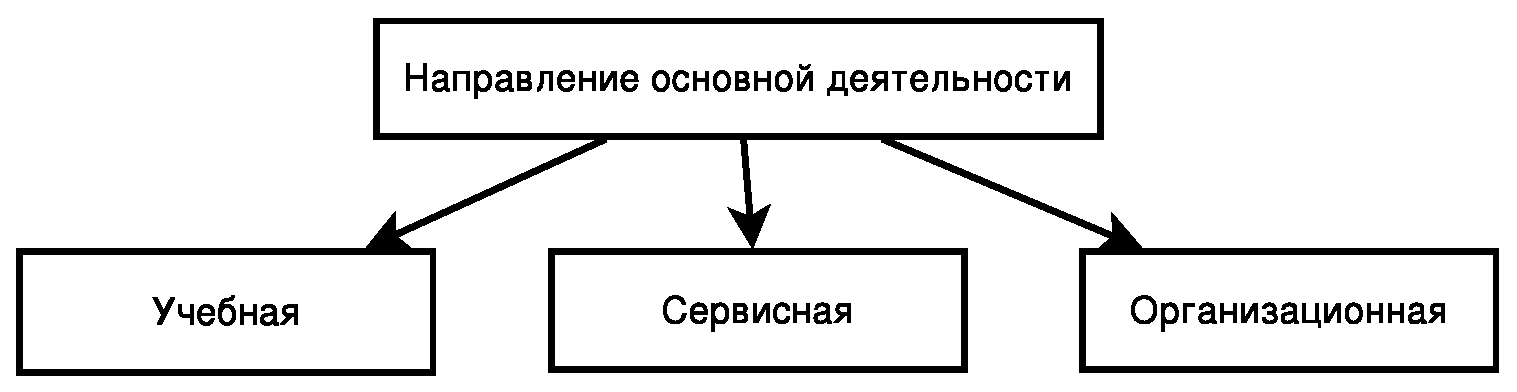
\includegraphics[height=160mm, width=0.8\textwidth, clip, keepaspectratio]{pictures/org_custom.eps}
   \caption{Направления деятельности сотрудников}\label{fig:org_custom}
 \end{figure}

У каждого работника СПбГДТЮ свой род занятий, обязанности и функции(Рисунок \ref{fig:org_custom}), следовательно, есть свои особенности и специфика .

В учебной деятельности это:
\begin{itemize}
\item Обилие документации;
\item Невозможность перерывов;
\item Сложность подготовки кадров при работе с информационной системой (ИС), так как многие сотрудники не готовы перейти на новое программное обеспечение, в основном из-за консервативных соображений;
\end{itemize}

В сервисной деятельности это:
\begin{itemize}
\item Обилие документации;
\item Большой объем работ;
\item Необходимость ведения учета;
\item Сопротивление персонала.
\end{itemize}

В организационной деятельности это:
\begin{itemize}
\item Обилие документации;
\item Необходимость текущего перехода на новую ИС без остановки, так как это приведет к простою в работе, большим финансовым потерям, нарушению учебного процесса и подрыву престижа организации;
\item Сопротивление персонала, так как многие не готовы переучиваться на другую систему и осваивать новое ПО.
\end{itemize}

У педагогов в следствии недостатка времени и иногда отсутствия желания осваивать новый продукт могут возникнуть трудности при переходе на новую информационную систему. С другой стороны, педагоги – люди, которые умеют учиться, что является неоспоримым плюсом для более быстрой реализации концепции, также этот фактор может заменить отсутствие желания.

Кроме того, многие педагоги работают не только во Дворце, но и дома, где зачастую используется другое программное обеспечение, в большинстве случаев проприетарное. Следовательно, необходимо предоставить возможность доступа к служебной информации, методическим и др. материалам, необходимым для обеспечения профессиональной деятельности без привязки к определённым операционным системам.

Управленческий аппарат почти весь состоит из людей, которые не только не хотят учиться, но и, зачастую, не умеют это делать. У таких сотрудников нет желания менять устоявшийся бизнес-процесс, поэтому их приходиться заставлять переучиваться, используя административный ресурс, что накладывает жёсткие ограничения на сложность использования системы хранения файлов.

Сервисные сотрудники обладают большим количеством свободного времени,
но у них отсутствует желание работать, трудиться, им свойственна лень, поэтому им не хочется учиться, но процесс обучения у них происходит быстрее за счёт имеющихся знаний.

Во Дворце ежедневного находиться большое количество сотрудников, выполняющих свои непосредственные обязанности, поэтому функционирование Дворца является непрерывным процессом, поэтому его не только не следует приостанавливать,
а даже категорически не рекомендуется это делать.

Таким образом система сетевого доступа к файлам должна быть максимально простой с точки зрения пользователя, использовать стандартизованные решения, реализации которых есть под все популярные операционные системы и быть открытым программным обеспечением.

\subsection{Предположительные архитектурные решения и задачи информационной системы}
Задачей хранилища данных является хранение файлов пользователей, дерева каталогов, информации о пользователях и их правах доступа.

Бизнес логика реализуется на сервере приложений, в рамках которой обеспечивается:
\begin{itemize}

\item авторизация пользователей, 
\item предоставление требуемых файлов и каталогов для работы в соответствие с правами доступа, 
\item блокировка используемых файлов 
\item получение обновлённой версии с возможным получением предыдущих версий файла.
\item запись информации о действиях пользователей в рамках системы
 \end{itemize}

Таким образом требуется:
\begin{itemize}
\item ведение журнала активности пользователей
\item предоставление удобный доступ пользователя к файлам и директориям, на которые ему были установлены права доступа
\item осуществление разделения пользователей по ролям доступа
\end{itemize}

Исходя из требований к системе, предлагается трёхзвенная архитектура: Клиент -- сервер приложений -- хранилище данных.

\section{Обзор аналогов}
\subsection{Samba}

Samba — программа, которая позволяет обращаться к сетевым дискам на различных операционных системах по протоколу SMB/CIFS. 
Имеет клиентскую и серверную части. Является свободным программным обеспечением, выпущена под лицензией GPL.
Минусами данного варианта реализации является ориентированность на работу в локальной сети, отсутствие версионирования файлов(реализуется только с помощью версионных ФС, реализации которых в Linux недостаточно протестированы для применения в промышленной эксплуатации).

\subsection{FTP с разделением прав}

Данное решение сложно в настройке, использовании. У этого решения отсутствует возможность 
удалённой работы с файлами. Файлы требуется сначала загрузить на локальный диск, внести 
изменения и после этого загрузить обратно на сервер. При этом не сохраняется предыдущая версия файла. При использовании такого решения, сложно получать информацию об изменениях прав доступа, модификациях файлов и дерева каталогов. Версионность доступа реализуется с только с помощью версионных ФС.

\subsection{Системы управления версиями}
Система управления версиями — программное обеспечение для облегчения работы с изменяющейся информацией. Система управления версиями позволяет хранить несколько версий одного и того же документа, при необходимости, возвращаться к более ранним версиям, определять, кто и когда сделал то или иное изменение и многое другое.

Системы контроля версий такие как: git, svn, cvs; требуют определённой подготовки от пользователя. Это решение требует от пользователя ручного получения файлов из хранилища и помещения их обратно. Невозможно ограничить глубину сохранения версий файлов, что при использовании не-текстовых данных приводит к быстрому разрастанию хранилища файлов.

\section{Формализация техического задания}
\subsection{Платформы}
\subsection{Средства}
\subsection{Функциональные ограничения}

Требуется ведение журнала активности пользователей, включающего в себя информацию о следующих действиях: 
\begin{itemize}
\item дату и время входа/выхода пользователя
\item создание файла
\item модификация файла
\item удаление файла
\item установка блокировки на файл
\item снятие блокировки с файла
\end{itemize}

Требуется предоставить удобный доступ пользователя к файлам и директориям, на которые ему были установлены права доступа такие как: чтение, запись, удаление файлов и каталогов.

Требуется разработать инструмент позволяющий:	
\begin{itemize}
\item получать информацию об изменениях произошедших с последнего входа пользователя в систему	
\item выполнять аутентификацию пользователя по логину/паролю	
\item выполнять подключение рабочей области пользователя в дерево каталогов
\end{itemize}

Необходимо осуществлять разделение пользователей по следующим ролям:	
\begin{itemize}
\item Пользователь 	в соответствие со своими правами имеет 	доступ к файлам и каталогам подразделения и к общим каталогам. Имеет доступ к предыдущим версиям своих файлов на чтение. 		
\item Администратор подразделения может назначать права 	доступа для сотрудников подразделения, создавать и удалять каталоги в каталоге подразделения. Имеет доступ на чтение к предыдущим версиям файлов подразделения	
\item Администратор создает и удаляет учётные записи пользователей, записи подразделений, назначает права доступа, имеет полный 	доступ к дереву каталогов, имеет полный 	доступ к предыдущим версиям файлов.
\end{itemize}

\chapter{Глава 2. Проектирование}
\section{Системные архитектурные решения}
\subsection{Распределение задач между компонентами}

\subsection{Описание задач решаемых отдельными компонентами}
\subsection{Описание интерфейсов между компонентами}

\section{Архитектура программы}
\subsection{Архитектура БД}
\begin{figure}[ht]
   \centering%центрируем картинку
   \includegraphics[height=160mm, width=0.8\textwidth, clip, keepaspectratio]{pictures/DB.eps}
   \caption{Схема БД}\label{fig:db_scheme}
 \end{figure}
\subsection{Архитектура клиентской части}
\subsection{Архитектура сервера приложений}
\section{Проектирование инфраструктуры}
\subsection{Оценка требований к серверу}
\subsection{Оценка требований к рабочему месту пользователя}
\subsection{Оценка требований к пропускной способности канала}

\chapter{Глава 3. Реализация}
\section{Особенности реализации БД}
\section{Особенности реализации инструмента администрирования}
\section{Особенности реализации клиентской части}
\section{Особенности тестирования и отладки}
\section{План внедрения и отладки}
\subsection{Организационные мероприятия}
\subsection{Технические мероприятия}
\subsection{Мероприятия сопровождения}

\chapter{Глава 4. Экономическая часть}
\chapter{Глава 5. Безопасность}

\Conclusion
заключение

\end{document}